\documentclass{article}[12pt]
\usepackage{graphicx} % Required for inserting images
\usepackage{listings}
\usepackage{hyperref}
\usepackage{tabularx}
\usepackage{float}
\usepackage{subfig}
\usepackage[a4paper, total={6in, 8in}]{geometry}

\title{EARIN Lab 3 Report}
\author{Krzysztof Rudnicki, 307585 \\ Jakub Kliszko, 303866  }
\date{\today}

\begin{document}

\maketitle
\section{Exercise Variant 2 - Predicting wine quality}
Our task was to write a program that predicts wine quality based on data containing: \\
fixed acidity,volatile acidity,citric acid,residual sugar,chlorides,free sulfur dioxide,total sulfur dioxide,density,pH,sulphates,alcohol,quality


\section{Implementation}
Program can be ran by installing python, moving to project directory and issuing command:
\begin{lstlisting}[language=bash]
python main.py
\end{lstlisting}
We have decided on implementing Linear and Logistical regression methods as we found them the easiest to implement \\  
There will be 3 types of output \\ 
\begin{enumerate}
    \item Number of wines with given quality (Graphical)
    \item How a given parameter impacts quality (Graphical)
    \item How well did linear and logistical regression performed (Textual)
\end{enumerate}
Upon clicking any button the next plot will be shown
\section{Results}
We have successfully implemented program to predict wine quality \\ 
\subsection{Data investigation}
There are 11 features in total and 1599 instances of those features \\ 
It is clear that there is an inbalance in quality of wines with majority of wines being either '5' or '6':
\begin{figure}[H]
    \caption{Plot showing inbalance in quality of wine}
    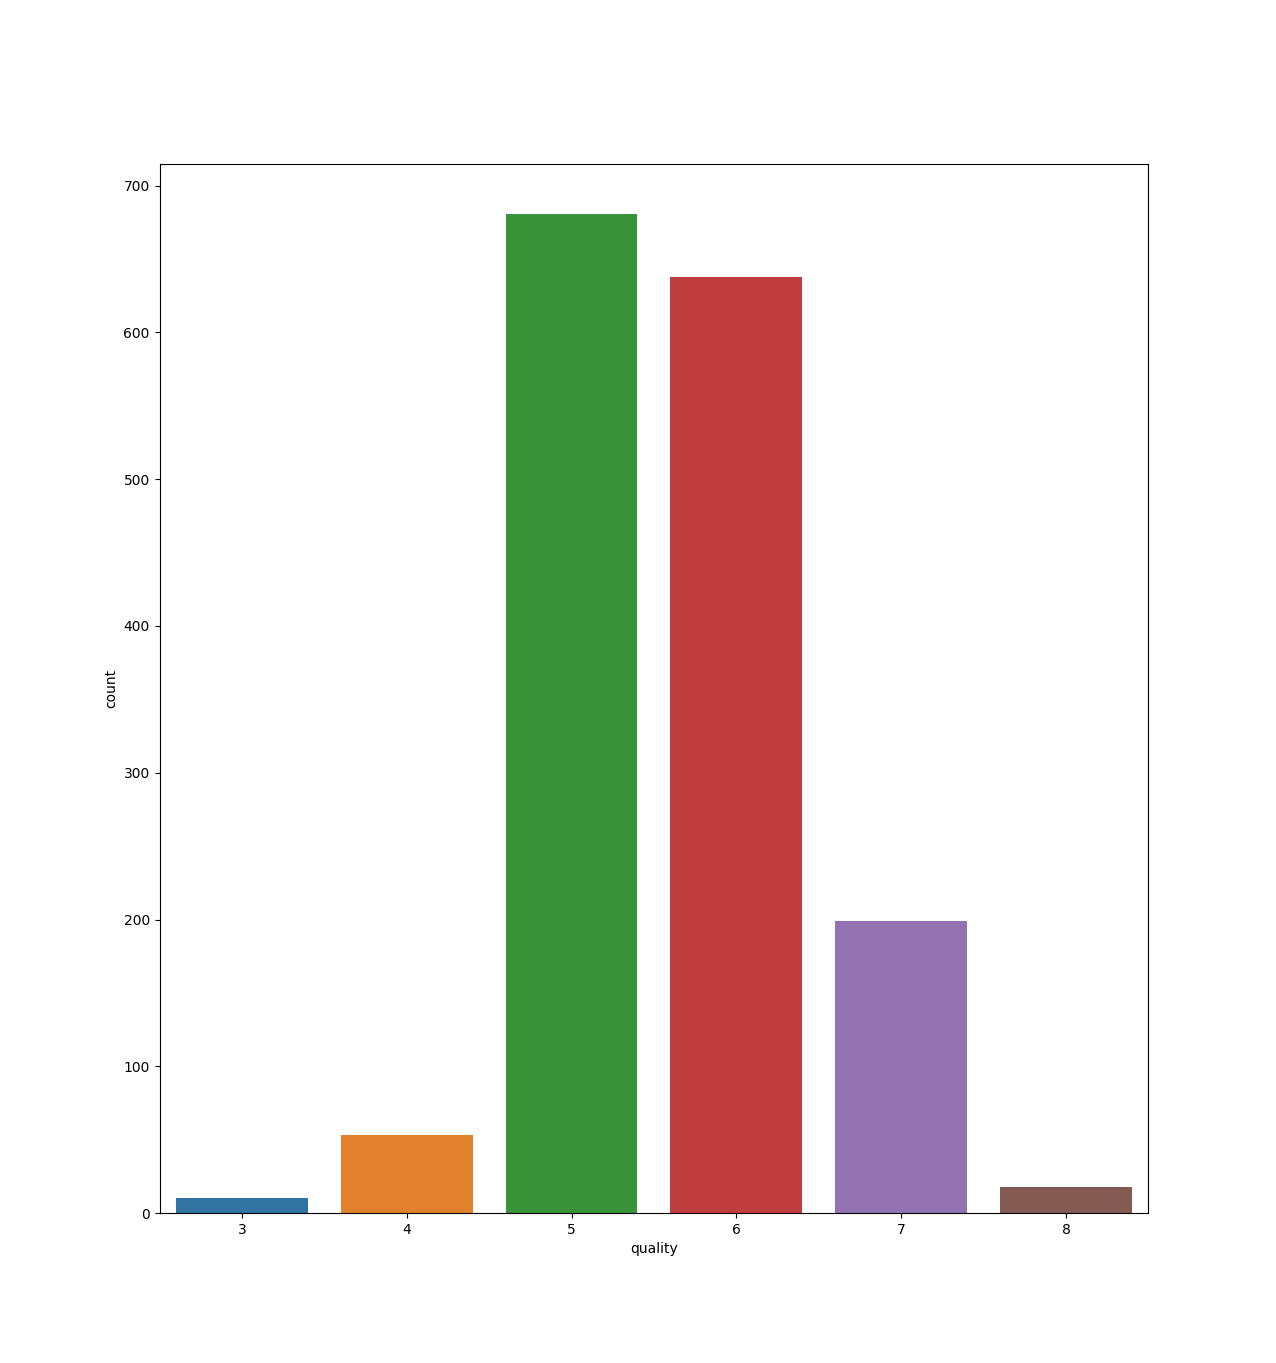
\includegraphics[width=\textwidth]{inbalance.png}
    \centering
    \end{figure}
More importantly we checked correlation of parameters:
\begin{figure}[H]
    \caption{Plot showing correlation between parameters, bright squares are positve correleation, dark squares are negative correleation}
    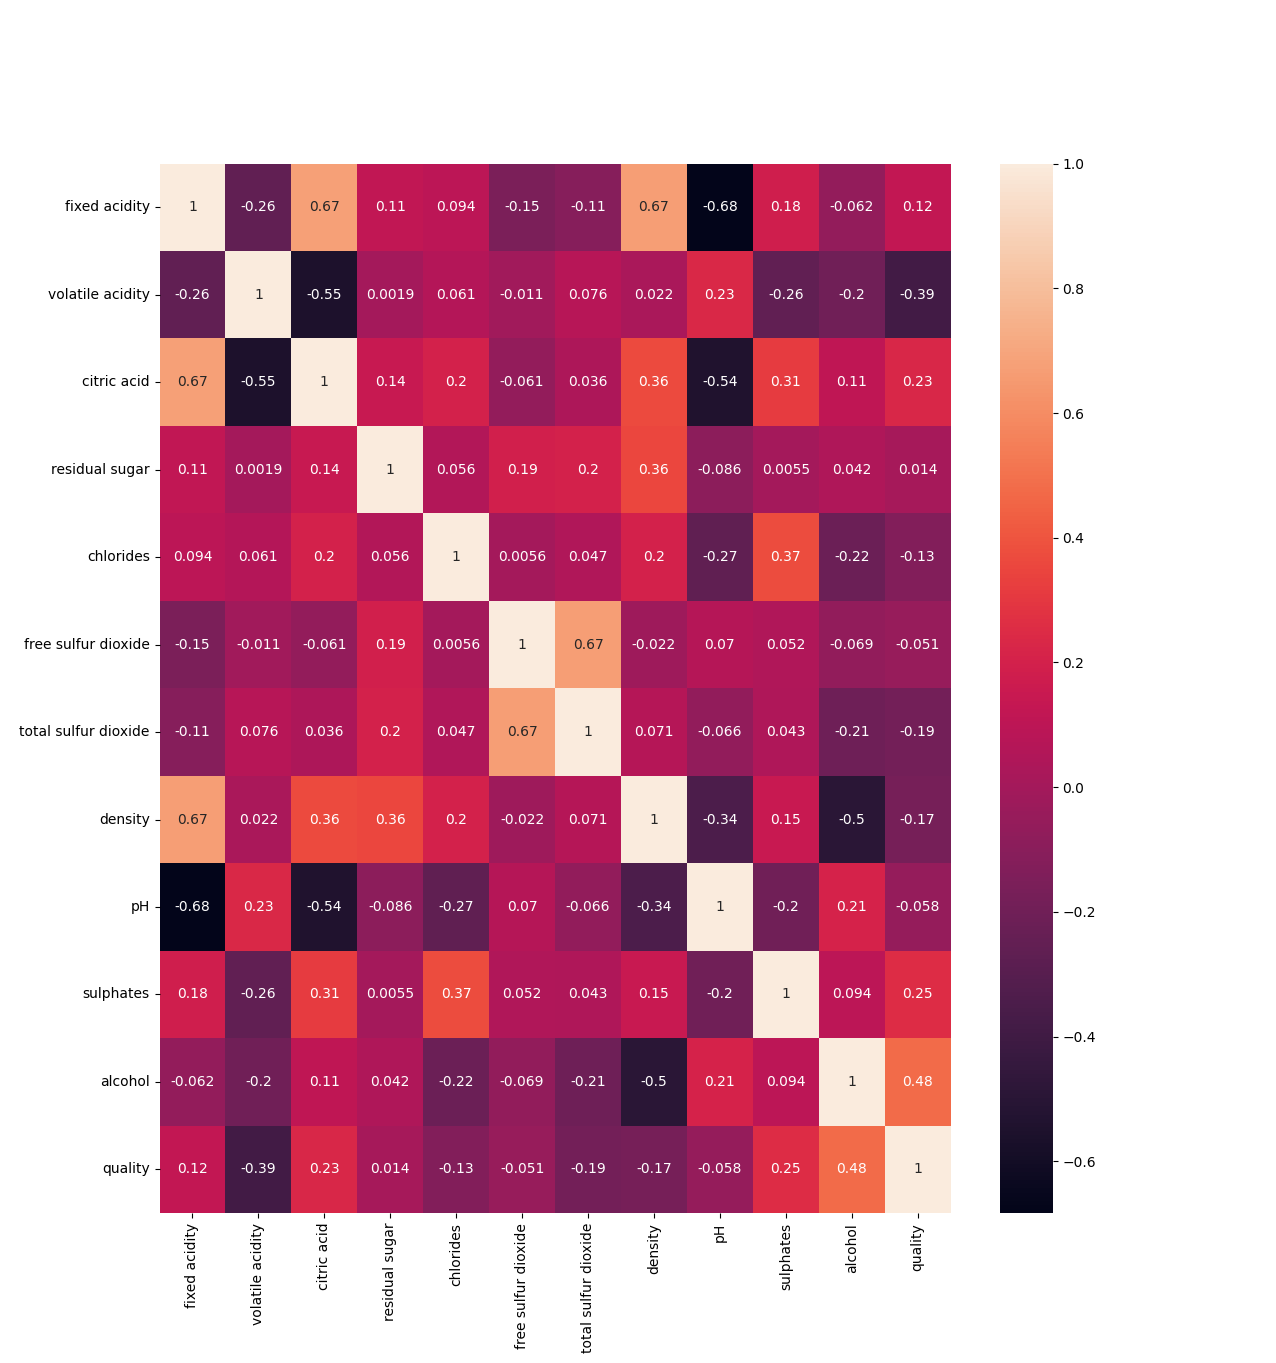
\includegraphics[width=\textwidth]{corr.png}
    \centering
    \end{figure}
Bright squares mean that the parameters have positive correlation to each other \\ 
Darker squares mean that the parameters have negative correlation to each other \\ 
\newpage
We are most intrested in correleation of certain parameters to quality value \\ 
Alcohol has by far the biggest positive impact on quality with coreleation value of 0.48 (where value of 1 means that those two parameters are equal to eachother), then we have sulphates and citric acid with roughly the same values (0.25 and 0.23 respectively) \\ 
The worst impact on quality is done by volatile acidity (-0.39)
\subsection{Methods comparison}
For Linear regression we checked values of:
\begin{itemize}
    \item Training Mean squared error - Difference between predicted and true values, the lower the better
    \item Training $R^2$ - for given data, The higher the better 
    \item Testing $R^2$ - for new data, The higher the better
\end{itemize}

For Logistic regression we checked values of:
\begin{itemize}
    \item Training Accuracy - how many instances we correctly classified, the higher the better 
    \item Training F1 Score - for given data, The higher the better 
    \item Testing F1 Score - for new data, The higher the better
\end{itemize}

For Linear regression we received values:
\begin{lstlisting}[language=bash]
Training MSE: 0.4258083784387746
Training R^2: 0.36545196162068627
Testing R^2: 0.3283887639580225
\end{lstlisting}

For Logistic regression we received values:
\begin{lstlisting}[language=bash]
Training Accuracy: 0.596559812353401
Training F1 Score: 0.5806169210603433
Testing F1 Score: 0.6166756344362352
\end{lstlisting}
We can see that Logistic regression outperforms linear regression, its test scores which is supposed to be as high as possible are twice as good as ones in linear regression 

\end{document}